\documentclass[final]{beamer}
%\usepackage[a1]{beamerposter}
\usetheme{umjiposter}
%\setlength{\paperwidth}{23.63in}
%\setlength{\paperheight}{35.44in}

%\setbeamercolor{block title}{fg=ngreen,bg=white} % Colors of the block titles
%\setbeamercolor{block body}{fg=black,bg=white} % Colors of the body of blocks
%\setbeamercolor{block alerted title}{fg=white,bg=dblue!70} % Colors of the highlighted block titles
%\setbeamercolor{block alerted body}{fg=black,bg=dblue!10} % Colors of the body of highlighted blocks

%\usepackage{booktabs} % Top and bottom rules for tables

%----------------------------------------------------------------------------------------
%	TITLE SECTION 
%----------------------------------------------------------------------------------------

\course{VE414 • Bayesian Analysis }
\title{Jiuling in the Forbidden Forest \\[.1in]} % Poster title
\author{Yanjun Zhou, Yangzhen Zhang, Yihao Liu} % Author(s)
\institute{Department and University Name} % Institution(s)
%\\sponsor{Shawn Ma, \textbf{\textit{Covidien}}}
%\advisor{Prof. Sung-Liang Chen}
\instructor{Prof. Jing Liu}

%----------------------------------------------------------------------------------------

\begin{document}

\addtobeamertemplate{block end}{}{\vspace*{2ex}} % White space under blocks
\addtobeamertemplate{block alerted end}{}{\vspace*{2ex}} % White space under highlighted (alert) blocks

\setlength{\belowcaptionskip}{2ex} % White space under figures
\setlength\belowdisplayshortskip{2ex} % White space under equations

\begin{frame}

\begin{columns}[t]

\begin{column}{\marginwidth}\end{column} % Empty spacer column

\begin{column}{\colwidth} % The first column
\begin{tcolorbox}[width=\colwidth,height=\contentheight,top=.2in]
\begin{block}{Problem Statement}
Jiuling trees, a kind of invisible plant, have been in the Forbidden Forest of Hogwarts for many years. With the help of a spell, number of the fruits of Jiuling, Tayes, are recorded along with the positions in some trips. This project is to visualize and analyze the data recorded by the spell and find the number and distribution of Jiuling in the Forbidden Forest. 
\vspace{.2in}

\begin{figure}[H]
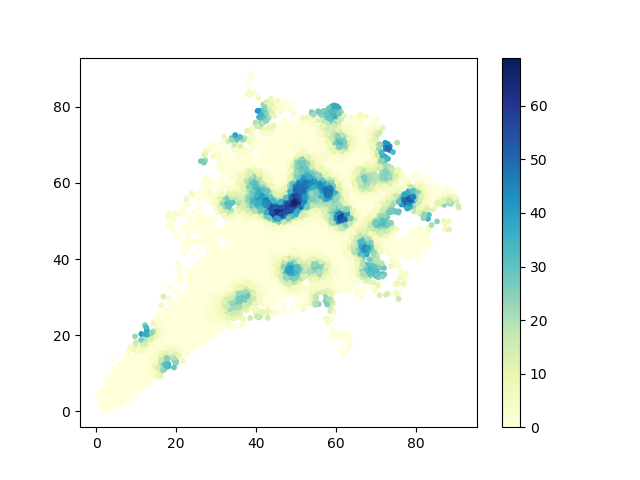
\includegraphics[width=0.9\textwidth]{ag}
\caption{A simple visualization of the data}
\end{figure}

\end{block}

\vspace{.2in}

\begin{block}{Density Estimation}
    Many records of Tayes $\implies$ Estimation of Tayes in the forest\\
    
    \begin{itemize}
        \item Divide map into grid 
        \begin{figure}[H]
        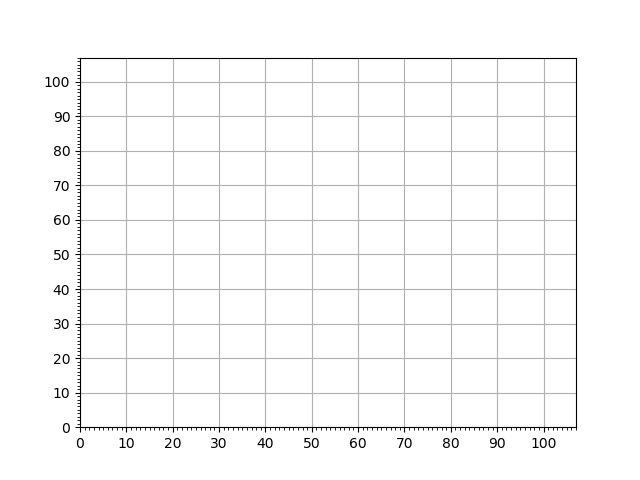
\includegraphics[width=0.7\textwidth]{grid}
        \end{figure}
        \item Calculate the density on the grid
        \begin{figure}[H]
        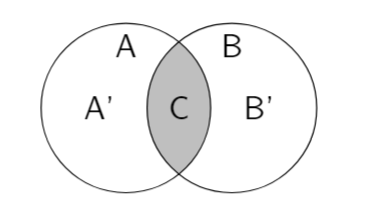
\includegraphics[width=0.7\textwidth]{circle.png}
        \end{figure}
        $$\quad\text{Density}[C]\approx\left(\frac{a}{S_A}+\frac{b}{S_B}\right)/2$$
        \item Sampling
    \end{itemize}
   

%\begin{figure}[H]
%\includegraphics[width=0.7\textwidth]{example-image-b}
%\caption{Detailed structure function}
%\end{figure}

\end{block}

\end{tcolorbox}
\end{column}

\begin{column}{\marginwidth-\parsep}\end{column} % Empty spacer column

\begin{column}{\colwidth} % The second column
\begin{tcolorbox}[width=\colwidth,height=\contentheight,top=.2in]

\begin{figure}[H]
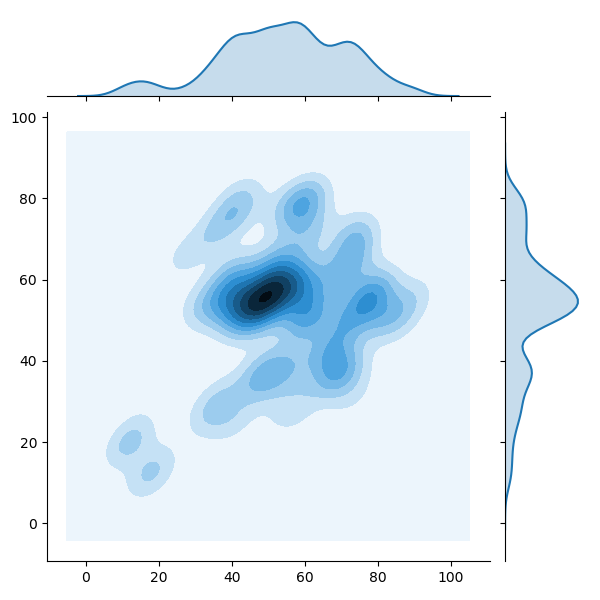
\includegraphics[width=0.9\textwidth]{density}
\caption{The density of Tayes over the forest with records}
\end{figure}

\begin{block}{GMM with EM}

Apply Expectation-Maximization algorithm (EM) to fit Guassian Mixture Model(GMM) with Tayes Samples.

    \begin{itemize}
        \item E-step: calculate the posterior probabilities for $k\in\{1,\cdots,K\}, n\in\{1,\cdots,N\}$ $$ \gamma_{nk}=p(k|x_n)=\dfrac{\pi_k\mathcal{N}(x_n|\mu_n,\Sigma_n)}{\sum_{j=1}^K\pi_j\mathcal{N}(x_n|\mu_j,\Sigma_j) } $$
        \item M-step: calculate the value for $\pi_k,\ \mu_k,\ \Sigma_k$
        \begin{align*}
            \mu_k' & = \dfrac{\sum_{n=1}^N\gamma_{nk}x_n}{\sum_{n=1}^N\gamma_{nk}}\\
            \Sigma_k' & = \dfrac{\sum_{n=1}^N\gamma_{nk}(x_n-\mu_k')(x_n-\mu_k')^T}{\sum_{n=1}^N\gamma_{nk}}\\
            \pi_k' &= \dfrac{\sum_{n=1}^N\gamma_{nk}}{N}
        \end{align*}
        \item Loop until log likelihood convergence:
        \begin{align*}
            & \text{ln}p(X|\mu,\Sigma,\pi)\\
            =&  \sum\limits_{n=1}^Nln\{\sum_{k=1}^K\pi_k\mathcal{N}(x_n|\mu_k,\Sigma_k)\}
        \end{align*}
        \item Pick a k = $\arg\limits_k\min$ BIC(Bayesian Information Creterion):
        $$ BIC = -2ln(L)+ln(N)*K $$
    \end{itemize}


\end{block}

\vspace{-.5in}



\end{tcolorbox}
\end{column}

\begin{column}{\marginwidth-\parsep}\end{column} % Empty spacer column

\begin{column}{\colwidth} % The third column
\begin{tcolorbox}[width=\colwidth,height=\contentheight,top=.2in]

By fitting the density with the Gaussian Mixture Model (GMM), we determined the number of the trees K as 72 based on Bayesian Information Criterion. The mean $\mu$ indicates the location of each tree. 

\vspace{.2in}

\begin{figure}[H]
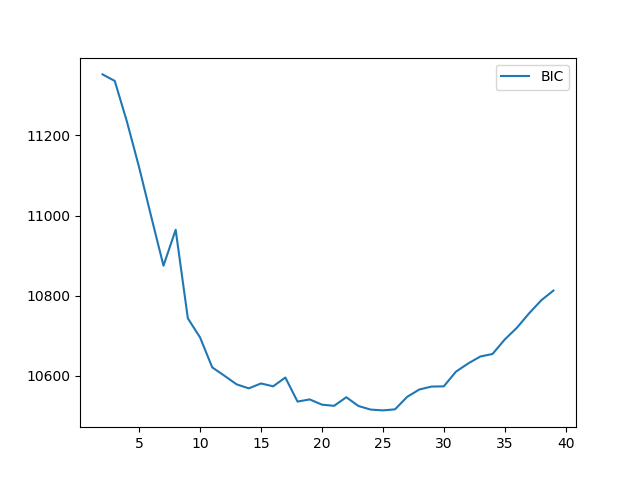
\includegraphics[width=0.9\textwidth]{bic}
\caption{BIC changes with K}
\end{figure}

\begin{figure}[H]
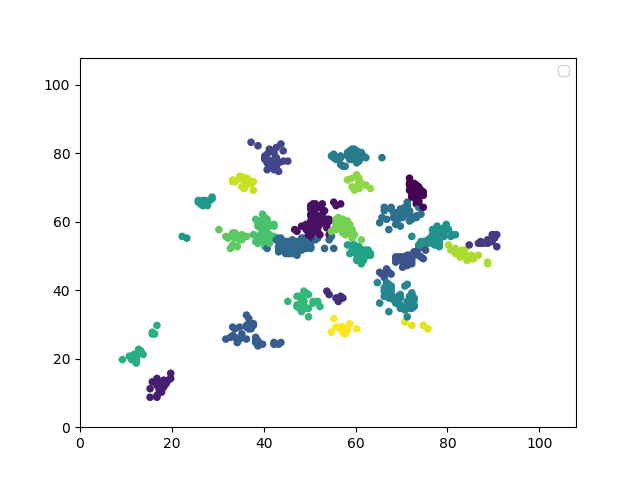
\includegraphics[width=0.9\textwidth]{trees}
\caption{An example for the tree distribution in the middle of the forest}
\end{figure}

\begin{block}{Prediction}

After we obtain a GMM for observed areas, we divide the forest into small grids and fit a model of tree density in each  related to its distances to two nearest borders of the forest. Therefore, we can predict the tree density of unobserved areas and make the final prediction of tree distribution and total tree number.

\begin{figure}[H]
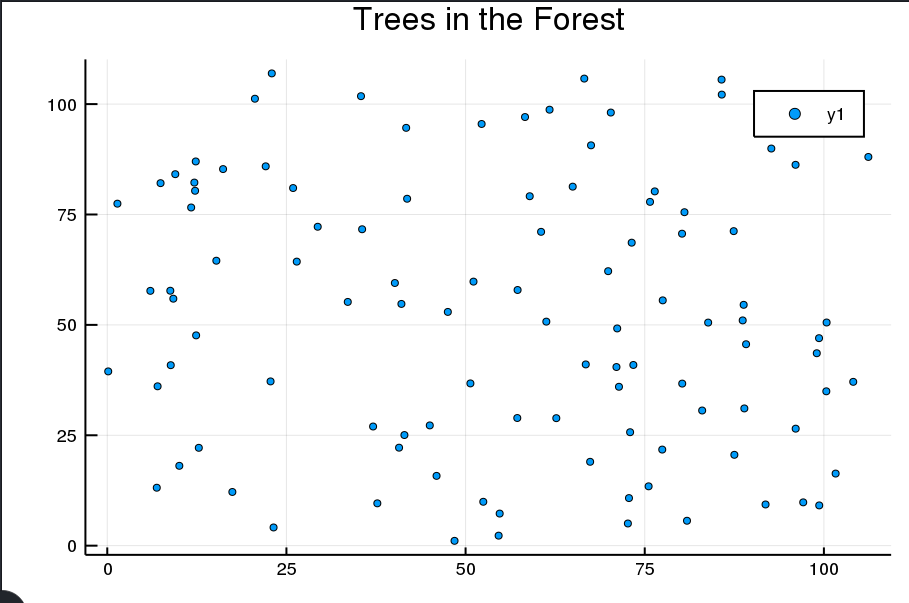
\includegraphics[width=0.9\textwidth]{predict}
\caption{Prediction of the trees in the forest}
\end{figure}
%加一张整个森林的图

\vspace{.2in}

\end{block}


%\begin{block}{Acknowledgement}
%\small Sponsor: Shawn Ma from Covidien

%Shane Johnson, Sung-Liang Chen and Huan Qi from UM-SJTU Joint Institute 

%Hongkun Lai and Xunjie Cai from UM-SJTU Joint Institute 
%\end{block}

%\begin{block}{Reference}
%\small 
%[1] \url{http://labs.seas.wustl.edu/bme/Wang/index.html}
%\end{block}


\end{tcolorbox}
\end{column}

\begin{column}{\marginwidth}\end{column} % Empty spacer column

\end{columns}

\end{frame}


%\begin{frame}[t] % The whole poster is enclosed in one beamer frame
%
%\begin{columns}[t] % The whole poster consists of three major columns, the second of which is split into two columns twice - the [t] option aligns each column's content to the top
%
%\begin{column}{\sepwid}\end{column} % Empty spacer column
%
%\begin{column}{\onecolwid} % The first column
%
%%----------------------------------------------------------------------------------------
%%	OBJECTIVES
%%----------------------------------------------------------------------------------------
%
%\begin{alertblock}{Objectives}
%
%Lorem ipsum dolor sit amet, consectetur, nunc tellus pulvinar tortor, commodo eleifend risus arcu sed odio:
%\begin{itemize}
%\item Mollis dignissim, magna augue tincidunt dolor, interdum vestibulum urna
%\item Sed aliquet luctus lectus, eget aliquet leo ullamcorper consequat. Vivamus eros sem, iaculis ut euismod non, sollicitudin vel orci.
%\item Nascetur ridiculus mus.  
%\item Euismod non erat. Nam ultricies pellentesque nunc, ultrices volutpat nisl ultrices a.
%\end{itemize}
%
%\end{alertblock}
%
%%----------------------------------------------------------------------------------------
%%	INTRODUCTION
%%----------------------------------------------------------------------------------------
%
%\begin{block}{Introduction}
%
%Lorem ipsum dolor \textbf{sit amet}, consectetur adipiscing elit. Sed commodo molestie porta. Sed ultrices scelerisque sapien ac commodo. Donec ut volutpat elit. Sed laoreet accumsan mattis. Integer sapien tellus, auctor ac blandit eget, sollicitudin vitae lorem. Praesent dictum tempor pulvinar. Suspendisse potenti. Sed tincidunt varius ipsum, et porta nulla suscipit et. Etiam congue bibendum felis, ac dictum augue cursus a. \textbf{Donec} magna eros, iaculis sit amet placerat quis, laoreet id est. In ut orci purus, interdum ornare nibh. Pellentesque pulvinar, nibh ac malesuada accumsan, urna nunc convallis tortor, ac vehicula nulla tellus eget nulla. Nullam lectus tortor, \textit{consequat tempor hendrerit} quis, vestibulum in diam. Maecenas sed diam augue.
%
%Lorem ipsum dolor \textbf{sit amet}, consectetur adipiscing elit. Sed commodo molestie porta. Sed ultrices scelerisque sapien ac commodo. Donec ut volutpat elit. Sed laoreet accumsan mattis. Integer sapien tellus, auctor ac blandit eget, sollicitudin vitae lorem. Praesent dictum tempor pulvinar. Suspendisse potenti. Sed tincidunt varius ipsum, et porta nulla suscipit et. Etiam congue bibendum felis, ac dictum augue cursus a.
%
%This statement requires citation \cite{Smith:2012qr}.
%
%\end{block}
%
%%------------------------------------------------
%
%\begin{figure}
%\includegraphics[width=0.8\linewidth]{placeholder.jpg}
%\caption{Figure caption}
%\end{figure}
%
%%----------------------------------------------------------------------------------------
%
%\end{column} % End of the first column
%
%\begin{column}{\sepwid}\end{column} % Empty spacer column
%
%\begin{column}{\twocolwid} % Begin a column which is two columns wide (column 2)
%
%\begin{columns}[t,totalwidth=\twocolwid] % Split up the two columns wide column
%
%\begin{column}{\onecolwid}\vspace{-.6in} % The first column within column 2 (column 2.1)
%
%%----------------------------------------------------------------------------------------
%%	MATERIALS
%%----------------------------------------------------------------------------------------
%
%\begin{block}{Materials}
%
%The following materials were required to complete the research:
%
%\begin{itemize}
%\item Curabitur pellentesque dignissim
%\item Eu facilisis est tempus quis
%\item Duis porta consequat lorem
%\item Eu facilisis est tempus quis
%\end{itemize}
%
%The materials were prepared according to the steps outlined below:
%
%\begin{enumerate}
%\item Curabitur pellentesque dignissim
%\item Eu facilisis est tempus quis
%\item Duis porta consequat lorem
%\item Curabitur pellentesque dignissim
%\end{enumerate}
%
%\end{block}
%
%%----------------------------------------------------------------------------------------
%
%\end{column} % End of column 2.1
%
%\begin{column}{\onecolwid}\vspace{-.6in} % The second column within column 2 (column 2.2)
%
%%----------------------------------------------------------------------------------------
%%	METHODS
%%----------------------------------------------------------------------------------------
%
%\begin{block}{Methods}
%
%Lorem ipsum dolor \textbf{sit amet}, consectetur adipiscing elit. Sed laoreet accumsan mattis. Integer sapien tellus, auctor ac blandit eget, sollicitudin vitae lorem. Praesent dictum tempor pulvinar. Suspendisse potenti. Sed tincidunt varius ipsum, et porta nulla suscipit et. Etiam congue bibendum felis, ac dictum augue cursus a. \textbf{Donec} magna eros, iaculis sit amet placerat quis, laoreet id est. In ut orci purus, interdum ornare nibh. Pellentesque pulvinar, nibh ac malesuada accumsan, urna nunc convallis tortor, ac vehicula nulla tellus eget nulla. Nullam lectus tortor, \textit{consequat tempor hendrerit} quis, vestibulum in diam. Maecenas sed diam augue.
%
%\end{block}
%
%%----------------------------------------------------------------------------------------
%
%\end{column} % End of column 2.2
%
%\end{columns} % End of the split of column 2 - any content after this will now take up 2 columns width
%
%%----------------------------------------------------------------------------------------
%%	IMPORTANT RESULT
%%----------------------------------------------------------------------------------------
%
%\begin{alertblock}{Important Result}
%
%Lorem ipsum dolor \textbf{sit amet}, consectetur adipiscing elit. Sed commodo molestie porta. Sed ultrices scelerisque sapien ac commodo. Donec ut volutpat elit.
%
%\end{alertblock} 
%
%%----------------------------------------------------------------------------------------
%
%\begin{columns}[t,totalwidth=\twocolwid] % Split up the two columns wide column again
%
%\begin{column}{\onecolwid} % The first column within column 2 (column 2.1)
%
%%----------------------------------------------------------------------------------------
%%	MATHEMATICAL SECTION
%%----------------------------------------------------------------------------------------
%
%\begin{block}{Mathematical Section}
%
%Nam quis odio enim, in molestie libero. Vivamus cursus mi at nulla elementum sollicitudin. Nam quis odio enim, in molestie libero. Vivamus cursus mi at nulla elementum sollicitudin.
%  
%\begin{equation}
%E = mc^{2}
%\label{eqn:Einstein}
%\end{equation}
%
%Nam quis odio enim, in molestie libero. Vivamus cursus mi at nulla elementum sollicitudin. Nam quis odio enim, in molestie libero. Vivamus cursus mi at nulla elementum sollicitudin.
%
%\begin{equation}
%\cos^3 \theta =\frac{1}{4}\cos\theta+\frac{3}{4}\cos 3\theta
%\label{eq:refname}
%\end{equation}
%
%Nam quis odio enim, in molestie libero. Vivamus cursus mi at nulla elementum sollicitudin. Nam quis odio enim, in molestie libero. Vivamus cursus mi at nulla elementum sollicitudin.
%
%\begin{equation}
%\kappa =\frac{\xi}{E_{\mathrm{max}}} %\mathbb{ZNR}
%\end{equation}
%
%Nam quis odio enim, in molestie libero. Vivamus cursus mi at nulla elementum sollicitudin. Nam quis odio enim, in molestie libero. Vivamus cursus mi at nulla elementum sollicitudin.
%
%\end{block}
%
%%----------------------------------------------------------------------------------------
%
%\end{column} % End of column 2.1
%
%\begin{column}{\onecolwid} % The second column within column 2 (column 2.2)
%
%%----------------------------------------------------------------------------------------
%%	RESULTS
%%----------------------------------------------------------------------------------------
%
%\begin{block}{Results}
%
%\begin{figure}
%\includegraphics[width=0.8\linewidth]{placeholder.jpg}
%\caption{Figure caption}
%\end{figure}
%
%Nunc tempus venenatis facilisis. Curabitur suscipit consequat eros non porttitor. Sed a massa dolor, id ornare enim:
%
%Nunc tempus venenatis facilisis. Curabitur suscipit consequat eros non porttitor. Sed a massa dolor, id ornare enim:
%
%Nunc tempus venenatis facilisis. Curabitur suscipit consequat eros non porttitor. Sed a massa dolor, id ornare enim:
%
%Nunc tempus venenatis facilisis. Curabitur suscipit consequat eros non porttitor. Sed a massa dolor, id ornare enim:
%
%\begin{table}
%\vspace{2ex}
%\begin{tabular}{l l l}
%\toprule
%\textbf{Treatments} & \textbf{Res. 1} & \textbf{Res. 2}\\
%\midrule
%Treatment 1 & 0.0003262 & 0.562 \\
%Treatment 2 & 0.0015681 & 0.910 \\
%Treatment 3 & 0.0009271 & 0.296 \\
%\bottomrule
%\end{tabular}
%\caption{Table caption}
%\end{table}
%
%\end{block}
%
%%----------------------------------------------------------------------------------------
%
%\end{column} % End of column 2.2
%
%\end{columns} % End of the split of column 2
%
%\end{column} % End of the second column
%
%\begin{column}{\sepwid}\end{column} % Empty spacer column
%
%\begin{column}{\onecolwid} % The third column
%
%%----------------------------------------------------------------------------------------
%%	CONCLUSION
%%----------------------------------------------------------------------------------------
%
%\begin{block}{Conclusion}
%
%Nunc tempus venenatis facilisis. \textbf{Curabitur suscipit} consequat eros non porttitor. Sed a massa dolor, id ornare enim. Fusce quis massa dictum tortor \textbf{tincidunt mattis}. Donec quam est, lobortis quis pretium at, laoreet scelerisque lacus. Nam quis odio enim, in molestie libero. Vivamus cursus mi at \textit{nulla elementum sollicitudin}.
%
%Nunc tempus venenatis facilisis. Curabitur suscipit consequat eros non porttitor. Sed a massa dolor, id ornare enim.
%
%\end{block}
%
%%----------------------------------------------------------------------------------------
%%	ADDITIONAL INFORMATION
%%----------------------------------------------------------------------------------------
%
%\begin{block}{Additional Information}
%
%Maecenas ultricies feugiat velit non mattis. Fusce tempus arcu id ligula varius dictum. 
%\begin{itemize}
%\item Curabitur pellentesque dignissim
%\item Eu facilisis est tempus quis
%\item Duis porta consequat lorem
%\end{itemize}
%
%Maecenas ultricies feugiat velit non mattis. Fusce tempus arcu id ligula varius dictum. 
%\begin{itemize}
%\item Curabitur pellentesque dignissim
%\item Eu facilisis est tempus quis
%\item Duis porta consequat lorem
%\end{itemize}
%
%\end{block}
%
%%----------------------------------------------------------------------------------------
%%	REFERENCES
%%----------------------------------------------------------------------------------------
%
%\begin{block}{References}
%
%\nocite{*} % Insert publications even if they are not cited in the poster
%\small{\bibliographystyle{unsrt}
%\bibliography{sample}\vspace{0.75in}}
%
%\end{block}
%
%%----------------------------------------------------------------------------------------
%%	ACKNOWLEDGEMENTS
%%----------------------------------------------------------------------------------------
%
%\setbeamercolor{block title}{fg=red,bg=white} % Change the block title color
%
%\begin{block}{Acknowledgements}
%
%\small{\rmfamily{Nam mollis tristique neque eu luctus. Suspendisse rutrum congue nisi sed convallis. Aenean id neque dolor. Pellentesque habitant morbi tristique senectus et netus et malesuada fames ac turpis egestas.}} \\
%
%\end{block}
%
%%----------------------------------------------------------------------------------------
%%	CONTACT INFORMATION
%%----------------------------------------------------------------------------------------
%
%\setbeamercolor{block alerted title}{fg=black,bg=norange} % Change the alert block title colors
%\setbeamercolor{block alerted body}{fg=black,bg=white} % Change the alert block body colors
%
%\begin{alertblock}{Contact Information}
%
%\begin{itemize}
%\item Web: \href{http://www.my.edu/smithlab}{http://www.my.edu/smithlab}
%\item Email: \href{mailto:john@smith.com}{john@smith.com}
%\item Phone: +1 (000) 111 1111
%\end{itemize}
%
%\end{alertblock}
%
%\begin{center}
%\begin{tabular}{ccc}
%\includegraphics[width=0.4\linewidth]{logo.png} & \hfill & \includegraphics[width=0.4\linewidth]{logo.png}
%\end{tabular}
%\end{center}
%
%%----------------------------------------------------------------------------------------
%
%\end{column} % End of the third column
%
%\end{columns} % End of all the columns in the poster
%
%\end{frame} % End of the enclosing frame
%
\end{document}
